\documentclass{amsart}
\usepackage[margin=3cm]{geometry}                % See geometry.pdf to learn the layout options. There are lots.
\geometry{letterpaper}                   % ... or a4paper or a5paper or ...
%\geometry{landscape}                % Activate for for rotated page geometry
\usepackage[parfill]{parskip}    % Activate to begin paragraphs with an empty line rather than an indent
\usepackage{float}
\usepackage[demo]{graphicx}
\usepackage{amssymb}
\usepackage{epstopdf}
\usepackage{siunitx}
\usepackage{subcaption}
\usepackage{units}
\usepackage{setspace}

\DeclareGraphicsRule{.tif}{png}{.png}{`convert #1 `dirname #1`/`basename #1 .tif`.png}
\graphicspath{{./img/}}

\title{Electron Spin Resonance}
\author{Caspar \textsc{Lant}} % Author name

\date{\today} % Date for the report

\begin{document}

\bigskip

\maketitle % Insert the title, author and date
\begin{center}

Intermediate Experimental Physics II\\
\vspace{1.5cm}

\begin{tabular}{l r}

Section: & 001\\
\\
Date Performed: & March 15, 2016 \\ % Date the experiment was performed
Date Due: & March 22, 2016\\
\\
Partner: & Neil Saddler\\ % Partner names
Professor: & Prof. Andrew Kent\\
Instructor: & David Mykytyn % Instructor/supervisor
\end{tabular}
\vfill
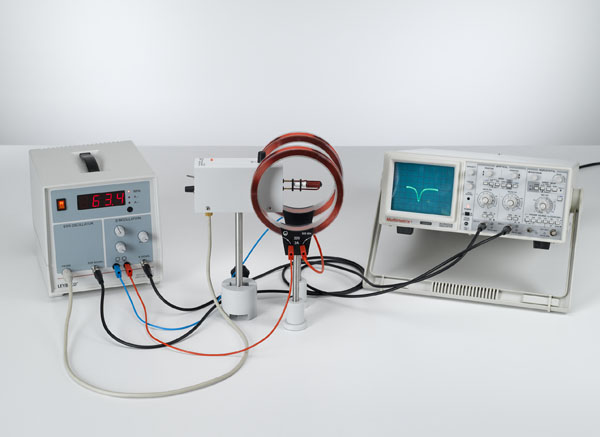
\includegraphics[width=.7\textwidth]{diagram.jpg}
\end{center}
\vfill
\pagebreak

\setstretch{1.5}
\paragraph{\textbf{The Objective} of this lab was to observe the famous photoelectric effect first hand, and to experimentally derive the value of Planck's constant, a quantity central to the study of quantum physics.   }

\section{Theoretical Background/ Abstract}
Due to quenching, the role of the orbital angular momentum of the paramagnetic electron in a DPPH molecule is very small. To begin with, we assume it is zero, and then will modify our expressions slightly at the end. The electron has a spin angular momentum S⃗ whose
magnitude is given by S = 􏰛s(s + 1)h ̄ where s = 1 is the spin quantum number. Associated 2
with S⃗ is a spin magnetic moment given by μ⃗ = −(gsμBS⃗)/h ̄, where gs is the g factor for the
electron’s spin and μB is the Bohr magneton. From this relation it is seen that gs, which is
dimensionless, is the ratio of the electron’s magnetic moment in units of the Bohr magneton
to its angular momentum in units of h ̄. We will take gs = 2 although if Q.E.D. corrections
are included it is equal to about 2.0023. It is twice gl, the g factor for the orbital motion.
In a magnetic field that points in the z direction the spin angular momentum can only have
projections onto the z-axis of Sz = h ̄ms, where ms is the magnetic spin quantum number
with values of only ±1. As a result the spin magnetic moment can only have projections onto 2
the magnetic field of μz = −gsμBms. As the potential energy of a dipole μ⃗ in a magnetic field B⃗ is U = −μ⃗ · B⃗, there are two possible energy levels whose values are ±1gsμBB. The
2
energy of these levels is plotted as a function of the magnetic field in Fig. 1. The energy difference △E between these two levels at a given magnetic field is
\begin{equation}
    \Delta E = h\nu = g\mu_B B
\end{equation}
where $\nu$ is the frequency of the radiation necessary to induce a transition and the subscript s has been removed from the g to account for the fact that there are still small effects due to the electron’s orbital motion and that we do not expect g to be exactly equal to 2. The value of g is measured in this experiment.
In an ESR experiment the line width can supply information about many properties. Contributions to the line width can come from
If we take $V_S$, the stopping potential, to be the kinetic energy of a given photoelectron times its charge, we can produce the following equation:
\begin{equation}
    V_s = \dfrac{h}{\rm e} \nu - \dfrac{\phi}{\rm e}
\end{equation}
In DPPH it is electron exchange which is important. The full width at half height of the resonance in terms of the magnetic field will be called $\delta B$ and will be measured.
\begin{equation}
    \vec \mu \times \vec B = \omega_L \times \vec L
\end{equation}

\begin{equation}
    \dfrac{\mu_0 N}{2R}\left(\dfrac{4}{5}\right)^{\frac{3}{2}}(2I_0) = 2.115(2I_0)mT
\end{equation}

\section{Experimental Procedure}
\begin{enumerate}
    \item Plug everything in in the manner depicted in the schematic.
    \item Now that I know that you don't read the procedure section, typing them up has become so much more laborious.
    \item Put on your pair of Ali-G glasses and instruct your partner to do the same.
    \item Remember, always don your pair of glasses first if your partner is unable to do so.
    \item Turn on the Ammeter (referred to in the lab manual as a galvenometer) and zero it.
    \item Zero both potentiometers such that the retarded voltage (displayed on the multimeter) is zero volts.
    \item Turn on the UV lamp and place it close to the device's aperture. Wait a minute and note the deflection on the ammeter.
    \item Turn the dial photoelectric effect device to the 577 nm wavelength position.
    \item Record the ammount of deflection by the ammeter for retarding voltages of zero to three volts, at tenth-of-a-volt intervals.
    \item Turn the dial to the next setting and repeat the last 3 steps.
    \item Repeat the last three steps for the remaining two wavelengths.
\end{enumerate}

\section{Graphs and Tables}

\begin{table}[H]
    \begin{minipage}{.45\textwidth}
\centering
\caption{Voltage vs. Deflection}
\bigskip \bigskip
\label{my-label}
\begin{tabular}{c|c|c|c}
    f (MHz) & Io (Amp) & 2Io (Amp) & B (mT) \\
    30.7    & 0.644    & 1.288     & 2.724  \\
    35.0    & 0.731    & 1.462     & 3.092  \\
    40.0    & 0.880    & 1.760     & 3.722  \\
    45.0    & 0.993    & 1.986     & 4.200  \\
    50.0    & 1.112    & 2.224     & 4.704  \\
    55.0    & 1.205    & 2.410     & 5.097  \\
    60.0    & 1.317    & 2.634     & 5.571  \\
    65.0    & 1.442    & 2.884     & 6.100  \\
    70.0    & 1.534    & 3.068     & 6.489  \\
    75.0    & 1.595    & 3.190     & 6.747  \\
    80.0    & 1.692    & 3.384     & 7.157  \\
    85.0    & 1.765    & 3.530     & 7.466  \\
    90.0    & 1.917    & 3.834     & 8.109  \\
    95.0    & 2.035    & 4.070     & 8.608  \\
    100.0   & 2.067    & 4.134     & 8.743  \\
    105.0   & 2.221    & 4.442     & 9.395  \\
    110.0   & 2.293    & 4.586     & 9.699  \\
    100.0   & 2.412    & 4.824     & 10.203
\end{tabular}
\end{minipage}
%
\begin{minipage}{.5\textwidth}
    \centering
    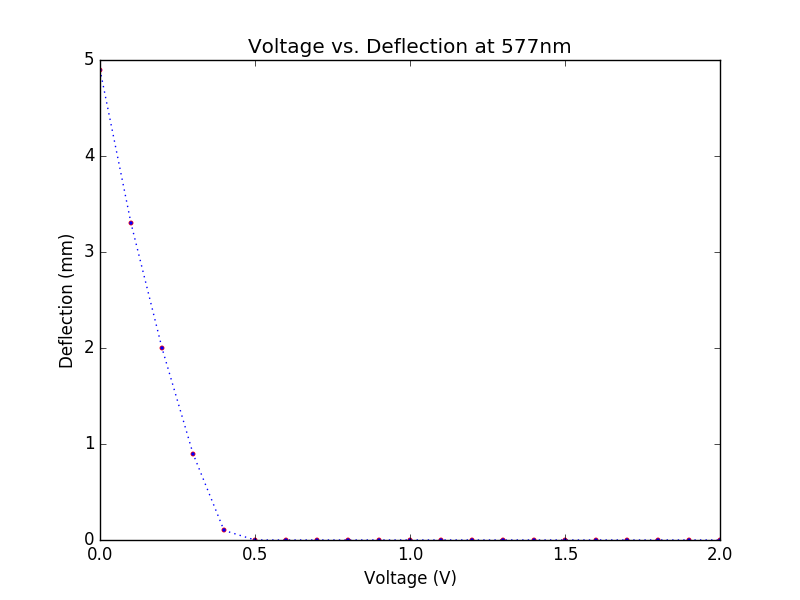
\includegraphics[height=.23\textheight]{577.png}\\
    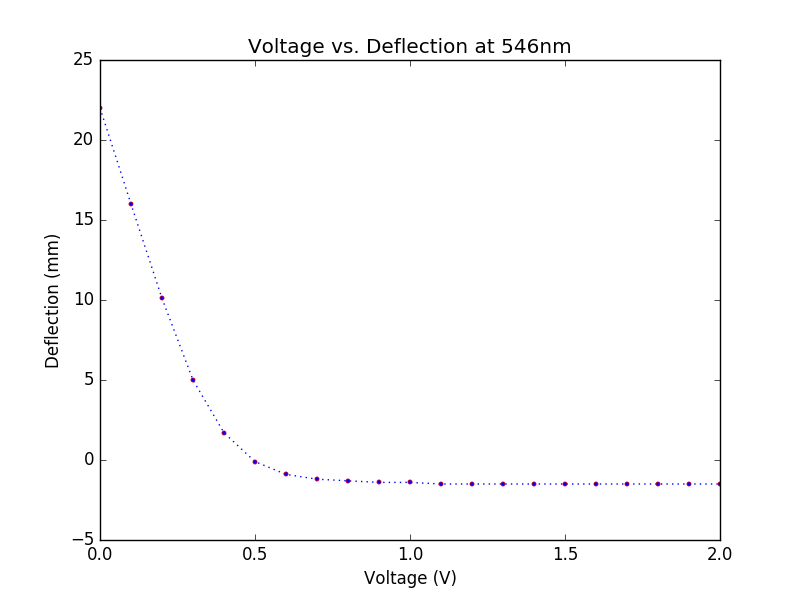
\includegraphics[height=.23\textheight]{546.png}\\
    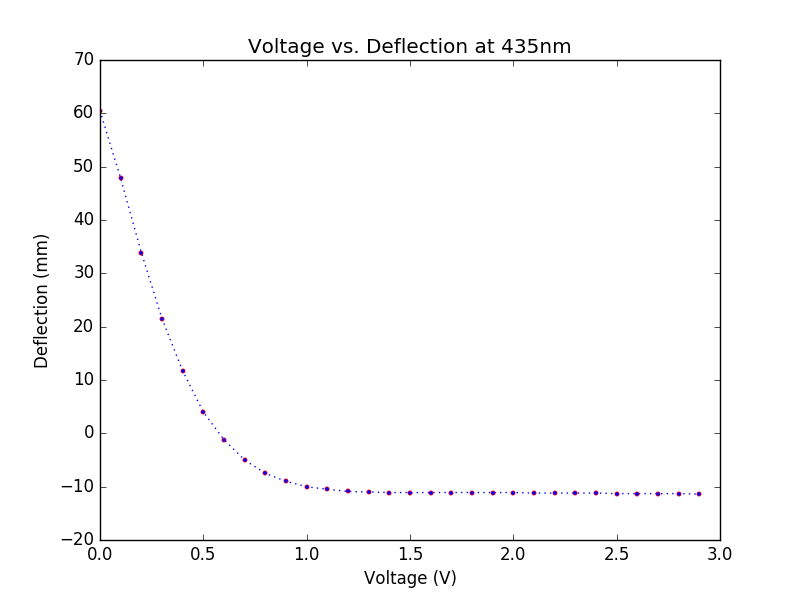
\includegraphics[height=.23\textheight]{435.png}
\end{minipage}
\end{table}

\begin{figure}
    \centering
    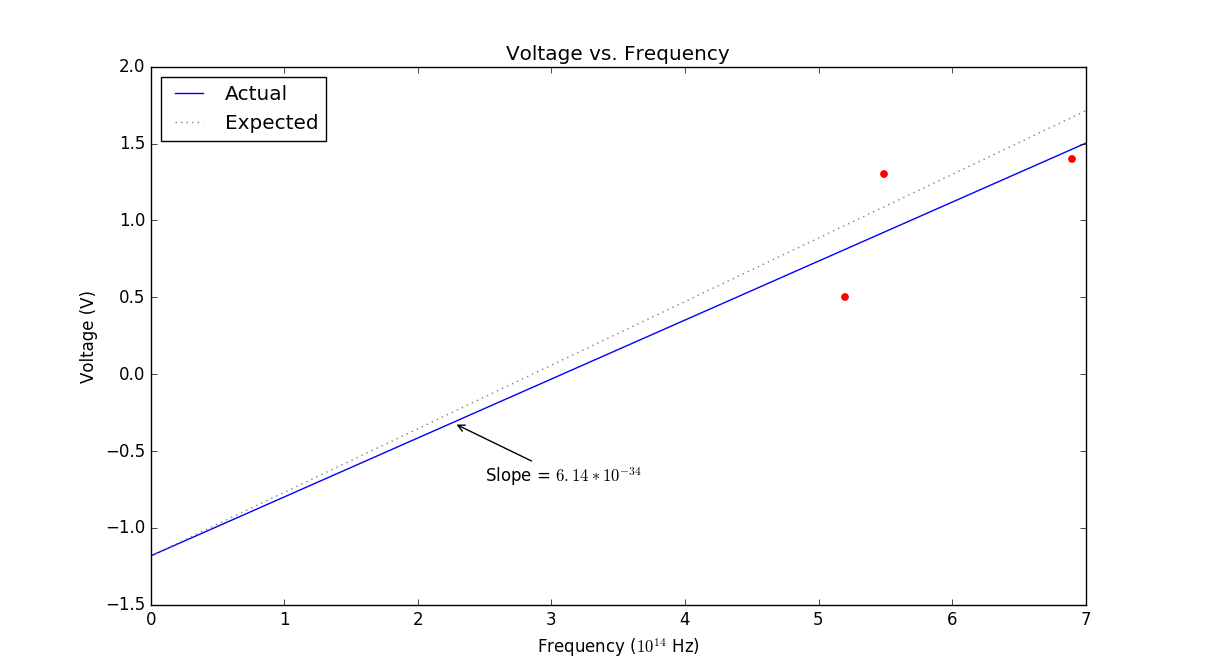
\includegraphics[width=\textwidth]{planckbest.png}
    \caption{Finding Planck's Constant}
    {$h = \unitfrac[6.14 \times 10^{-34}]{ m^2 kg}{s}$}
\end{figure}

\begin{figure}
    \centering
    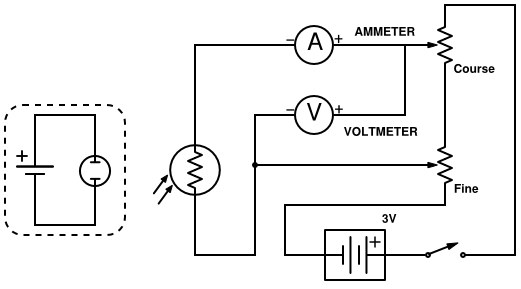
\includegraphics[width=0.8\textwidth]{schematic.png}
    \caption{Schematic Diagram of the Experimental Setup}
\end{figure}


\begin{figure}
    \begin{minipage}{.45\textwidth}
        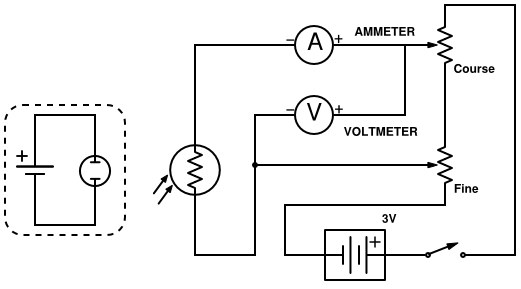
\includegraphics[width=\textwidth]{schematic.png}
    \end{minipage}
    %
    \begin{minipage}{.45\textwidth}

    \end{minipage}
\end{figure}

The topmost plot corresponds to a filter of slit width 577 nm, the middle plot 546 nm, and the last plot a wavelength of 435 nm.
\section{Questions}

\begin{enumerate}
    \item {\textit{The manufacturer designed this experiment with the coils connected in parallel. A series connection would be better. Why?}
    \begin{quote}
        There don't seem to be any questions to answer in this lab report.
    \end{quote}}
    \item {\textit{The p-p modulation current δ(2I0) for the half-width δB is obtained from  Where does the divisor 10 come from?}
    \begin{quote}

    \end{quote}}
    \item {\textit{In the method given for measuring δB, the scope controls are not used in a calibrated mode. Why is this OK?}
    \begin{quote}

    \end{quote}}
    \item {\textit{Why is the multimeter set for DC amperes for measuring g and for AC amperes for measuring the line width?}
    \begin{quote}

    \end{quote}}
    \item {\textit{Is there an RF electric field associated with the RF coil? If so, make a sketch of what the fields look like.}
    \begin{quote}

    \end{quote}}



\end{enumerate}

\section{Error Analysis}




\end{document}
